\documentclass[a4paper]{article}
\addtolength{\hoffset}{-2.25cm}
\addtolength{\textwidth}{4.5cm}
\addtolength{\voffset}{-3.25cm}
\addtolength{\textheight}{5cm}
\setlength{\parskip}{0pt}
\setlength{\parindent}{0in}

%----------------------------------------------------------------------------------------
%	PACKAGES AND OTHER DOCUMENT CONFIGURATIONS
%----------------------------------------------------------------------------------------

\usepackage{blindtext} % Package to generate dummy text
\usepackage[utf8]{inputenc} % Use UTF-8 encoding
\usepackage{microtype} % Slightly tweak font spacing for aesthetics
\usepackage[english]{babel} % Language hyphenation and typographical rules
\usepackage{amsthm, amsmath, amssymb} % Mathematical typesetting
\usepackage{mathtools} % Mathematical typesetting
\usepackage{float} % Improved interface for floating objects
\usepackage[final, colorlinks = true,
            linkcolor = black,
            citecolor = black]{hyperref} % For hyperlinks in the PDF
\usepackage{graphicx, multicol} % Enhanced support for graphics
\usepackage[dvipsnames]{xcolor} % Driver-independent color extensions
\usepackage{marvosym, wasysym} % More symbols
\usepackage{rotating} % Rotation tools
\usepackage{censor} % Facilities for controlling restricted text
\usepackage{listings, style/lstlisting} % Environment for non-formatted code, !uses style file!
\usepackage{pseudocode} % Environment for specifying algorithms in a natural way
\usepackage{style/avm} % Environment for f-structures, !uses style file!
\usepackage{booktabs} % Enhances quality of tables
\usepackage{bm} % Enhances quality of tables
\usepackage{tikz-qtree} % Easy tree drawing tool
\usepackage{enumitem} % enumerate with custom labels
\tikzset{every tree node/.style={align=center,anchor=north},
         level distance=2cm} % Configuration for q-trees
\usepackage{style/btree} % Configuration for b-trees and b+-trees, !uses style file!
\usepackage[backend=biber,style=numeric,
            sorting=nyt]{biblatex} % Complete reimplementation of bibliographic facilities
\addbibresource{ecl.bib}
\usepackage{csquotes} % Context sensitive quotation facilities
\usepackage[yyyymmdd]{datetime} % Uses YEAR-MONTH-DAY format for dates
\renewcommand{\dateseparator}{-} % Sets dateseparator to '-'
\usepackage{fancyhdr} % Headers and footers
\pagestyle{fancy} % All pages have headers and footers
\fancyhead{}\renewcommand{\headrulewidth}{0pt} % Blank out the default header
\fancyfoot[L]{} % Custom footer text
\fancyfoot[C]{} % Custom footer text
\fancyfoot[R]{\thepage} % Custom footer text
\newcommand{\note}[1]{\marginpar{\scriptsize \textcolor{red}{#1}}} % Enables comments in red on margin

%----------------------------------------------------------------------------------------

\newcommand*{\vertbar}{\rule[-1ex]{0.5pt}{2.5ex}}
\newcommand*{\horzbar}{\rule[.5ex]{2.5ex}{0.5pt}}

\newcommand{\E}[1]{{\mathbb{E}\left[#1\right]}}
\newcommand{\var}[1]{{\text{var}\left[#1\right]}}
\newcommand{\diffpart}[1]{\frac{\partial}{\partial #1}}
\newcommand{\diffpartt}[2]{\frac{\partial#1}{\partial #2}}
\newcommand{\?}{\stackrel{?}{=}}
\newcommand{\intinf}{\int\limits_{-\infty}^{\infty}}
\newcommand{\intnulinf}{\int\limits_{0}^{\infty}}
\newcommand{\intpi}{\int\limits_{0}^{2\pi}}
\newcommand{\sume}[1]{\sum\limits_{#1}}
\newcommand{\sumt}[2]{\sum\limits_{#1}^{#2}}
\newcommand{\prodt}[2]{\prod\limits_{#1}^{#2}}
\newcommand{\argmin}[1]{\underset{#1}{\mathop{\mathrm{argmin}}}}
\newcommand{\argmax}[1]{\underset{#1}{\mathop{\mathrm{argmax}}}}
\newcommand{\normdist}[1]{\mathcal{N}(#1)}
\newcommand{\half}{\frac{1}{2}}
\newcommand{\ind}[2]{\mathbb{I}(#1=#2)}
\renewcommand{\arraystretch}{1.3}

% VECTOR NOTATION
\newcommand{\mSig}{\bm{\Sigma}}
\newcommand{\mSigi}{\bm{\Sigma}^{-1}}
\newcommand{\mS}{\bm{S}}
\newcommand{\mX}{\mathbf{X}}
\newcommand{\mM}{\mathbf{M}}
\newcommand{\mV}{\mathbf{V}}
\newcommand{\mY}{\mathbf{Y}}
\newcommand{\mSi}{\bm{S}^{-1}}
\newcommand{\mI}{\mathbf{I}}
\newcommand{\mPhi}{\bm{\Phi}}
\newcommand{\vnul}{\bm{0}}
\newcommand{\vx}{\mathbf{x}}
\newcommand{\va}{\mathbf{a}}
\newcommand{\vw}{\mathbf{w}}
\newcommand{\vu}{\mathbf{u}}
\newcommand{\vy}{\mathbf{y}}
\newcommand{\vt}{\bm{t}}
\newcommand{\vxi}{\bm{\xi}}
\newcommand{\vmu}{\bm{\mu}}
\newcommand{\valpha}{\bm{\alpha}}
\newcommand{\vphi}{\bm{\phi}}
\newcommand{\vpi}{\bm{\pi}}
\newcommand{\vlambda}{\bm{\lambda}}
\newcommand{\Ck}{\mathcal{C}_k}
\newcommand{\mTheta}{\bm{\Theta}}
\newcommand{\mT}{\bm{T}}
\newcommand{\mW}{\bm{W}}
\newcommand{\vtheta}{\bm{\theta}}

% vim: ft=tex

\begin{document}

%-------------------------------
%   TITLE SECTION
%-------------------------------

\fancyhead[C]{}
\hrule \medskip % Upper rule
\begin{minipage}{0.295\textwidth}
    \raggedright
    \footnotesize
    Maico Timmerman \hfill\\
    10542590\hfill\\
    maico.timmerman@gmail.com
\end{minipage}
\begin{minipage}{0.4\textwidth}
    \centering
    \large
    Homework Assignment 3\\
    \normalsize
    Natural Language Processing 1, 17/18\\
\end{minipage}
\begin{minipage}{0.295\textwidth}
    \raggedleft
    \today\hfill\\
\end{minipage}
\medskip\hrule
\bigskip

%-------------------------------
%   CONTENTS
%-------------------------------

\newcommand{\CCG}[3][]{
\begin{tabular}[t]{@{\hspace{-3pt}}c@{\hspace{-3pt}}}
#2\\[-7pt]
\leavevmode \leaders \hrule \hskip 0pt plus 1filll \kern 0pt % <<< change
    \raisebox{-2.5pt}{\footnotesize{#1}}\\
    \begin{tabular}[t]{@{}c@{}}
        \textit{#3}
    \end{tabular}
\end{tabular}
}

\section*{Questions 1}
\CCG[$<$]{
    \CCG[$>$]{
        \CCG{The}{NP/\textcolor{BlueViolet}{N}}
        \CCG{company}{\textcolor{BlueViolet}{N}}
    }{\textcolor{CadetBlue}{NP}}
    \CCG[$<$]{
        \CCG[$>$]{
            \CCG[$>$]{
                \CCG{added}{((S\textbackslash NP) / PP) / \textcolor{RedOrange}{NP}}
                \CCG[$>$]{
                    \CCG{four}{NP/\textcolor{OliveGreen}{N}}
                    \CCG{Boeing-747s}{\textcolor{OliveGreen}{N}}
                }{\textcolor{RedOrange}{NP}}
            }{(S\textbackslash NP) / \textcolor{Cyan}{PP}}
            \CCG[$>$]{
                \CCG{to}{PP/\textcolor{Goldenrod}{NP}}
                \CCG[$>$]{
                    \CCG{the}{NP/\textcolor{Maroon}{N}}
                    \CCG[$>$]{
                        \CCG{two}{N/\textcolor{SpringGreen}{N}}
                        \CCG{units}{\textcolor{SpringGreen}{N}}
                    }{\textcolor{Maroon}{N}}
                }{\textcolor{Goldenrod}{NP}}
            }{\textcolor{Cyan}{PP}}
        }{\textcolor{Red}{S\textbackslash NP}}
        \CCG[$>$]{
            \CCG{in}{((S\textbackslash NP) \textbackslash (S \textbackslash NP))/\textcolor{MidnightBlue}{NP}}
            \CCG{1994}{\textcolor{MidnightBlue}{NP}}
        }{(S\textbackslash NP) \textbackslash \textcolor{Red}{S\textbackslash NP}}
    }{S\textbackslash \textcolor{CadetBlue}{NP}}
}{S}

\section*{Questions 2}
\begin{enumerate}
    \item

\begin{align}
    \ln (P(y \mid\vx)) &= \ln \left(\frac{1}{Z}\exp\left(\sumt{i}{}w_if_i(\vx, y)\right)\right)\\
    &=-\ln(Z) + \sumt{i}{}w_if_i(\vx, y))\\
\end{align}

where $Z$ is defined as the normalization constant:
$\sumt{y'}{}\exp\left(\sumt{i}{}w_if_i(\vx, y')\right)$

We can work with log probabilities the same way we work with normal probabilities, as the same linear operators can be applied in log space as in the standard space.

\item
    \begin{align}
        y=1 :\sumt{i}{}w_if_i(\vx, y) &= 2.0\cdot f_1 -0.1\cdot f_7 &(\text{Other $f_i$ are 0})\\
        &= 2.0\cdot 1 -0.1\cdot 1= 1.9\\
        y=2 :\sumt{i}{}w_if_i(\vx, y) &= 1.8\cdot f_2 + 1.1\cdot f_8 &(\text{Other $f_i$ are 0})\\
        &= 1.8\cdot 1 + 1.1\cdot 1= 2.9\\
        y=3 :\sumt{i}{}w_if_i(\vx, y) &= 0.3\cdot f_3 + 2.7\cdot f_9 &(\text{Other $f_i$ are 0})\\
        &= 0.3\cdot 1 + 2.7\cdot 1= 3.0
    \end{align}

    We then calculate the value for the normalization constant $Z$:

    \begin{align}
        Z &= \sumt{y'}{}\exp\left(\sumt{i}{}w_if_i(\vx, y')\right)\\
        &= \exp(1.9) + \exp(2.9) + \exp(3.0)
        &= 44.946
    \end{align}

    The value for $P(y\mid\vx)$ the becomes:

    \begin{align}
        P(y=1\mid\vx) &= \frac{\exp\left(\sume{i}w_if_i(\vx, y)\right)}{Z}\\
        &= \frac{\exp(1.9)}{Z}\\
        &\approx 0.149\\
        P(y=2\mid\vx) &= \frac{\exp\left(\sumt{i}{}w_if_i(\vx, y)\right)}{Z}\\
        &= \frac{\exp(2.9)}{Z}\\
        &\approx 0.404\\
        P(y=3\mid\vx) &= \frac{\exp\left(\sumt{i}{}w_if_i(\vx, y)\right)}{Z}\\
        &= \frac{\exp(3.0)}{Z}\\
        &\approx 0.447
    \end{align}

\end{enumerate}

\section*{Questions 3}
    \begin{enumerate}
        \item All bears are furry.
        \item Sergii is eating pizza with a fork.
        \item All students are lifting Marie
        \item Marie is only lifted by students.
    \end{enumerate}

\section*{Questions 4}
    \begin{enumerate}
        \item
            \begin{align}
                \forall x.pasta(x) \Rightarrow hates(Juan, x)
            \end{align}
        \item
            \begin{align}
                \exists x. student(x) \land \forall y.class(y) \Rightarrow likes(x, y)
            \end{align}
    \end{enumerate}

\section*{Questions 5}

    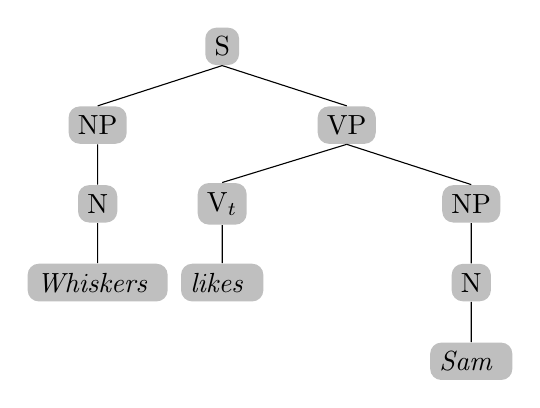
\begin{tikzpicture}[sibling distance=9em,
        level distance=1.0cm,
        every node/.style = {shape=rectangle, rounded corners,
            align=center, fill=black!25}]]
        \node {S}
            child { node {NP}
                child { node {N}
                    child { node { \textit{Whiskers} } } } }
            child { node {VP}
                child { node {V$_t$}
                    child { node { \textit{likes} } } }
                child { node {NP}
                    child { node {N}
                        child { node { \textit{Sam} } } } } };
    \end{tikzpicture}

    Below we have explained the semantics bottom up:
    \begin{alignat}{4}
        N_1.sem &&&= \text{Wiskers}\\
        N_2.sem &&&= \text{Sam}\\
        V_t.sem &&&= \lambda x.\lambda y.\exists e.Linging(e) \land Liker(e, y) \land Likee(e, x)\\
        NP_1.sem &= N_1.sem &&= \text{Wiskers}\\
        NP_2.sem &= N_2.sem &&= \text{Sam}\\
        VP.sem &= V_t.sem(NP.sem) &&= \lambda y.\exists e.Linging(e) \land Liker(e, y) \land Likee(e, \text{Sam})\\
        S.sem &= VP.sem(NP.sem) &&=\exists e.Linging(e) \land Liker(e,\text{Wiskers}) \land Likee(e, \text{Sam})
    \end{alignat}


\end{document}
% vim: ft=tex tw=0
